\newcommand{\insertsmallteaser}[1]{
  \includegraphics[height=\height, trim={14em 2em 14em 0}, clip]{assets/\clogdirname/teaser/teaser_scale=#1.png}
}
\newcommand{\insertsmalluv}[1]{
  \includegraphics[height=\smallheightuv]{assets/\clogdirname/teaser/uv_scale=#1.png}
}
\newcommand{\clogteasermanual}{
  \def\height{128bp}
  \def\smallheight{64bp}
  \def\smallheightuv{76bp}
  \begin{subfigure}[c]{\linewidth}
    \centering

    \tikzsetnextfilename{clogteaser}
    \tikzset{external/export next=false}
    \resizebox{\linewidth}{!}{
      \begin{tikzpicture}[
          >=stealth',
          overlay/.style={
              anchor=south west,
              draw=black,
              rectangle,
              line width=0pt,
              outer sep=0,
              inner sep=0,
            },
        ]

        \node (representation) {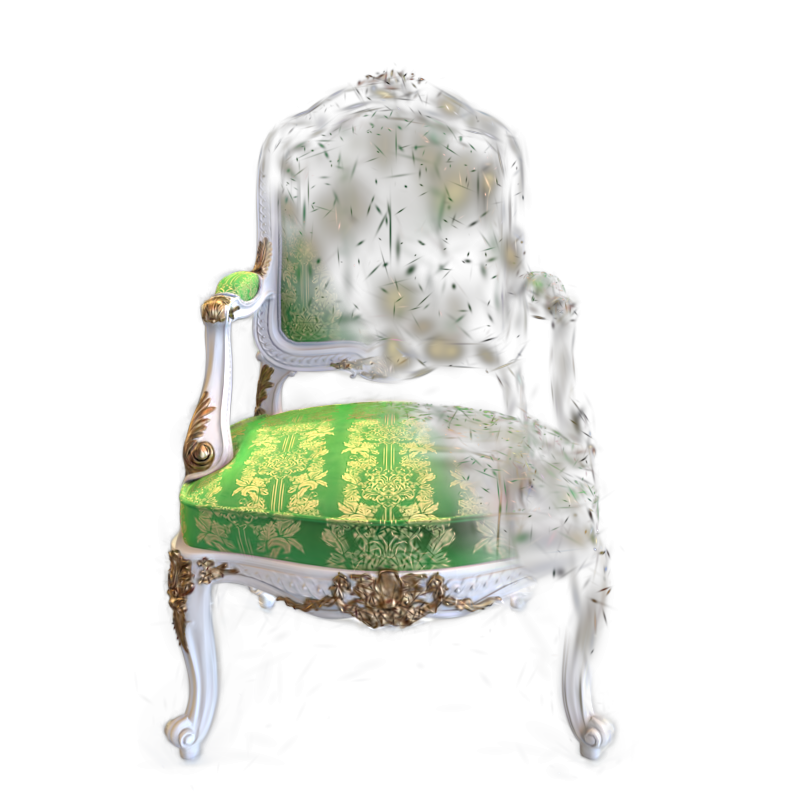
\includegraphics[height=\height, trim={12em 2em 12em 0}, clip]{assets/\clogdirname/teaser/teaser_1_blended.png}};
        \node[circle, thick, fill=white, draw, below left=4.5em and 1.25em of representation.south] (x1) {};
        \node[circle, thick, fill=white, draw, below=0.1em of x1] (x2) {};
        \node[circle, thick, fill=white, draw, below=0.1em of x2] (x3) {};
        \node[circle, thick, fill=white, draw, above=0.1em of x1] (x4) {};
        \node[circle, thick, fill=white, draw, above=0.1em of x4] (x5) {};

        \node[circle, thick, fill=white, draw, right=2em of x1] (x11) {};
        \node[circle, thick, fill=white, draw, below=0.1em of x11] (x12) {};
        \node[circle, thick, fill=white, draw, above=0.1em of x11] (x13) {};

        \foreach \x in {1,...,5}
        \foreach \y in {1,...,3}
        \draw (x\x) -- (x1\y);
        \matrix[
          matrix of nodes,
          right=1em of representation,
          column sep=0pt,
          row sep=0pt,
          ampersand replacement=\&,
          inner sep=0,
          outer sep=0
        ] (pictures) {
          \insertsmallteaser{0.1} \&
          \insertsmallteaser{0.25} \&
          \insertsmallteaser{0.5} \&
          % \insertsmallteaser{0.75} \&
          \insertsmallteaser{1.0} \\
        };

        \node[below=1em of pictures-1-1.south, outer sep=2pt] (uv1) {\insertsmalluv{0.1}};
        \node[below=1em of pictures-1-2.south, outer sep=2pt] (uv2) {\insertsmalluv{0.25}};
        \node[below=1em of pictures-1-3.south, outer sep=2pt] {\insertsmalluv{0.5}};
        \node[below=1em of pictures-1-4.south, outer sep=2pt] (uv5) {\insertsmalluv{1.0}};
        \draw[-stealth, shorten <=2pt, decoration={snake}, decorate, thick] (x11) -- node [midway, above, outer sep=3pt] {\tiny modulation} (uv1);

        \node[above=0em of pictures, anchor=base] (novelview) {Novel view and level of details synthesis};
        \node[above=-0.5em of representation, anchor=base, align=center] {Learned\\representation};

        \node[below=0em of pictures, align=center] {Learned 2D grid of features};

        \draw[-stealth,  thick, dashed, ->] (uv1.south west) -- node [below, midway] {Increasing Continuous Levels of Details} (uv5.south east);

        \node[below=0.5em of representation.south] {Modulator~$\modulator$};
        \node[above right=2em and 0em of pictures.south east, anchor=west, scale=0.85] (plot) {%% Creator: Matplotlib, PGF backend
%%
%% To include the figure in your LaTeX document, write
%%   \input{<filename>.pgf}
%%
%% Make sure the required packages are loaded in your preamble
%%   \usepackage{pgf}
%%
%% Also ensure that all the required font packages are loaded; for instance,
%% the lmodern package is sometimes necessary when using math font.
%%   \usepackage{lmodern}
%%
%% Figures using additional raster images can only be included by \input if
%% they are in the same directory as the main LaTeX file. For loading figures
%% from other directories you can use the `import` package
%%   \usepackage{import}
%%
%% and then include the figures with
%%   \import{<path to file>}{<filename>.pgf}
%%
%% Matplotlib used the following preamble
%%   \def\mathdefault#1{#1}
%%   \everymath=\expandafter{\the\everymath\displaystyle}
%%   
%%   \ifdefined\pdftexversion\else  % non-pdftex case.
%%     \usepackage{fontspec}
%%   \fi
%%   \makeatletter\@ifpackageloaded{underscore}{}{\usepackage[strings]{underscore}}\makeatother
%%
\begingroup%
\makeatletter%
\begin{pgfpicture}%
\pgfpathrectangle{\pgfpointorigin}{\pgfqpoint{4.000000in}{4.000000in}}%
\pgfusepath{use as bounding box}%
\begin{pgfscope}%
\pgfsetbuttcap%
\pgfsetmiterjoin%
\definecolor{currentfill}{rgb}{1.000000,1.000000,1.000000}%
\pgfsetfillcolor{currentfill}%
\pgfsetlinewidth{0.000000pt}%
\definecolor{currentstroke}{rgb}{1.000000,1.000000,1.000000}%
\pgfsetstrokecolor{currentstroke}%
\pgfsetdash{}{0pt}%
\pgfpathmoveto{\pgfqpoint{0.000000in}{0.000000in}}%
\pgfpathlineto{\pgfqpoint{4.000000in}{0.000000in}}%
\pgfpathlineto{\pgfqpoint{4.000000in}{4.000000in}}%
\pgfpathlineto{\pgfqpoint{0.000000in}{4.000000in}}%
\pgfpathlineto{\pgfqpoint{0.000000in}{0.000000in}}%
\pgfpathclose%
\pgfusepath{fill}%
\end{pgfscope}%
\begin{pgfscope}%
\pgfsetbuttcap%
\pgfsetmiterjoin%
\definecolor{currentfill}{rgb}{1.000000,1.000000,1.000000}%
\pgfsetfillcolor{currentfill}%
\pgfsetlinewidth{0.000000pt}%
\definecolor{currentstroke}{rgb}{0.000000,0.000000,0.000000}%
\pgfsetstrokecolor{currentstroke}%
\pgfsetstrokeopacity{0.000000}%
\pgfsetdash{}{0pt}%
\pgfpathmoveto{\pgfqpoint{0.500000in}{0.440000in}}%
\pgfpathlineto{\pgfqpoint{3.600000in}{0.440000in}}%
\pgfpathlineto{\pgfqpoint{3.600000in}{3.520000in}}%
\pgfpathlineto{\pgfqpoint{0.500000in}{3.520000in}}%
\pgfpathlineto{\pgfqpoint{0.500000in}{0.440000in}}%
\pgfpathclose%
\pgfusepath{fill}%
\end{pgfscope}%
\begin{pgfscope}%
\pgfpathrectangle{\pgfqpoint{0.500000in}{0.440000in}}{\pgfqpoint{3.100000in}{3.080000in}}%
\pgfusepath{clip}%
\pgfsetroundcap%
\pgfsetroundjoin%
\pgfsetlinewidth{1.003750pt}%
\definecolor{currentstroke}{rgb}{0.800000,0.800000,0.800000}%
\pgfsetstrokecolor{currentstroke}%
\pgfsetdash{}{0pt}%
\pgfpathmoveto{\pgfqpoint{0.640509in}{0.440000in}}%
\pgfpathlineto{\pgfqpoint{0.640509in}{3.520000in}}%
\pgfusepath{stroke}%
\end{pgfscope}%
\begin{pgfscope}%
\definecolor{textcolor}{rgb}{0.150000,0.150000,0.150000}%
\pgfsetstrokecolor{textcolor}%
\pgfsetfillcolor{textcolor}%
\pgftext[x=0.640509in,y=0.308056in,,top]{\color{textcolor}{\rmfamily\fontsize{13.750000}{16.500000}\selectfont\catcode`\^=\active\def^{\ifmmode\sp\else\^{}\fi}\catcode`\%=\active\def%{\%}$\mathdefault{0}$}}%
\end{pgfscope}%
\begin{pgfscope}%
\pgfpathrectangle{\pgfqpoint{0.500000in}{0.440000in}}{\pgfqpoint{3.100000in}{3.080000in}}%
\pgfusepath{clip}%
\pgfsetroundcap%
\pgfsetroundjoin%
\pgfsetlinewidth{1.003750pt}%
\definecolor{currentstroke}{rgb}{0.800000,0.800000,0.800000}%
\pgfsetstrokecolor{currentstroke}%
\pgfsetdash{}{0pt}%
\pgfpathmoveto{\pgfqpoint{1.715712in}{0.440000in}}%
\pgfpathlineto{\pgfqpoint{1.715712in}{3.520000in}}%
\pgfusepath{stroke}%
\end{pgfscope}%
\begin{pgfscope}%
\definecolor{textcolor}{rgb}{0.150000,0.150000,0.150000}%
\pgfsetstrokecolor{textcolor}%
\pgfsetfillcolor{textcolor}%
\pgftext[x=1.715712in,y=0.308056in,,top]{\color{textcolor}{\rmfamily\fontsize{13.750000}{16.500000}\selectfont\catcode`\^=\active\def^{\ifmmode\sp\else\^{}\fi}\catcode`\%=\active\def%{\%}$\mathdefault{100000}$}}%
\end{pgfscope}%
\begin{pgfscope}%
\pgfpathrectangle{\pgfqpoint{0.500000in}{0.440000in}}{\pgfqpoint{3.100000in}{3.080000in}}%
\pgfusepath{clip}%
\pgfsetroundcap%
\pgfsetroundjoin%
\pgfsetlinewidth{1.003750pt}%
\definecolor{currentstroke}{rgb}{0.800000,0.800000,0.800000}%
\pgfsetstrokecolor{currentstroke}%
\pgfsetdash{}{0pt}%
\pgfpathmoveto{\pgfqpoint{2.790916in}{0.440000in}}%
\pgfpathlineto{\pgfqpoint{2.790916in}{3.520000in}}%
\pgfusepath{stroke}%
\end{pgfscope}%
\begin{pgfscope}%
\definecolor{textcolor}{rgb}{0.150000,0.150000,0.150000}%
\pgfsetstrokecolor{textcolor}%
\pgfsetfillcolor{textcolor}%
\pgftext[x=2.790916in,y=0.308056in,,top]{\color{textcolor}{\rmfamily\fontsize{13.750000}{16.500000}\selectfont\catcode`\^=\active\def^{\ifmmode\sp\else\^{}\fi}\catcode`\%=\active\def%{\%}$\mathdefault{200000}$}}%
\end{pgfscope}%
\begin{pgfscope}%
\definecolor{textcolor}{rgb}{0.150000,0.150000,0.150000}%
\pgfsetstrokecolor{textcolor}%
\pgfsetfillcolor{textcolor}%
\pgftext[x=2.050000in,y=0.082917in,,top]{\color{textcolor}{\rmfamily\fontsize{15.000000}{18.000000}\selectfont\catcode`\^=\active\def^{\ifmmode\sp\else\^{}\fi}\catcode`\%=\active\def%{\%}\# Gaussians}}%
\end{pgfscope}%
\begin{pgfscope}%
\pgfpathrectangle{\pgfqpoint{0.500000in}{0.440000in}}{\pgfqpoint{3.100000in}{3.080000in}}%
\pgfusepath{clip}%
\pgfsetroundcap%
\pgfsetroundjoin%
\pgfsetlinewidth{1.003750pt}%
\definecolor{currentstroke}{rgb}{0.800000,0.800000,0.800000}%
\pgfsetstrokecolor{currentstroke}%
\pgfsetdash{}{0pt}%
\pgfpathmoveto{\pgfqpoint{0.500000in}{0.723707in}}%
\pgfpathlineto{\pgfqpoint{3.600000in}{0.723707in}}%
\pgfusepath{stroke}%
\end{pgfscope}%
\begin{pgfscope}%
\definecolor{textcolor}{rgb}{0.150000,0.150000,0.150000}%
\pgfsetstrokecolor{textcolor}%
\pgfsetfillcolor{textcolor}%
\pgftext[x=0.172225in, y=0.657440in, left, base]{\color{textcolor}{\rmfamily\fontsize{13.750000}{16.500000}\selectfont\catcode`\^=\active\def^{\ifmmode\sp\else\^{}\fi}\catcode`\%=\active\def%{\%}$\mathdefault{18}$}}%
\end{pgfscope}%
\begin{pgfscope}%
\pgfpathrectangle{\pgfqpoint{0.500000in}{0.440000in}}{\pgfqpoint{3.100000in}{3.080000in}}%
\pgfusepath{clip}%
\pgfsetroundcap%
\pgfsetroundjoin%
\pgfsetlinewidth{1.003750pt}%
\definecolor{currentstroke}{rgb}{0.800000,0.800000,0.800000}%
\pgfsetstrokecolor{currentstroke}%
\pgfsetdash{}{0pt}%
\pgfpathmoveto{\pgfqpoint{0.500000in}{1.110426in}}%
\pgfpathlineto{\pgfqpoint{3.600000in}{1.110426in}}%
\pgfusepath{stroke}%
\end{pgfscope}%
\begin{pgfscope}%
\definecolor{textcolor}{rgb}{0.150000,0.150000,0.150000}%
\pgfsetstrokecolor{textcolor}%
\pgfsetfillcolor{textcolor}%
\pgftext[x=0.172225in, y=1.044159in, left, base]{\color{textcolor}{\rmfamily\fontsize{13.750000}{16.500000}\selectfont\catcode`\^=\active\def^{\ifmmode\sp\else\^{}\fi}\catcode`\%=\active\def%{\%}$\mathdefault{20}$}}%
\end{pgfscope}%
\begin{pgfscope}%
\pgfpathrectangle{\pgfqpoint{0.500000in}{0.440000in}}{\pgfqpoint{3.100000in}{3.080000in}}%
\pgfusepath{clip}%
\pgfsetroundcap%
\pgfsetroundjoin%
\pgfsetlinewidth{1.003750pt}%
\definecolor{currentstroke}{rgb}{0.800000,0.800000,0.800000}%
\pgfsetstrokecolor{currentstroke}%
\pgfsetdash{}{0pt}%
\pgfpathmoveto{\pgfqpoint{0.500000in}{1.497145in}}%
\pgfpathlineto{\pgfqpoint{3.600000in}{1.497145in}}%
\pgfusepath{stroke}%
\end{pgfscope}%
\begin{pgfscope}%
\definecolor{textcolor}{rgb}{0.150000,0.150000,0.150000}%
\pgfsetstrokecolor{textcolor}%
\pgfsetfillcolor{textcolor}%
\pgftext[x=0.172225in, y=1.430878in, left, base]{\color{textcolor}{\rmfamily\fontsize{13.750000}{16.500000}\selectfont\catcode`\^=\active\def^{\ifmmode\sp\else\^{}\fi}\catcode`\%=\active\def%{\%}$\mathdefault{22}$}}%
\end{pgfscope}%
\begin{pgfscope}%
\pgfpathrectangle{\pgfqpoint{0.500000in}{0.440000in}}{\pgfqpoint{3.100000in}{3.080000in}}%
\pgfusepath{clip}%
\pgfsetroundcap%
\pgfsetroundjoin%
\pgfsetlinewidth{1.003750pt}%
\definecolor{currentstroke}{rgb}{0.800000,0.800000,0.800000}%
\pgfsetstrokecolor{currentstroke}%
\pgfsetdash{}{0pt}%
\pgfpathmoveto{\pgfqpoint{0.500000in}{1.883864in}}%
\pgfpathlineto{\pgfqpoint{3.600000in}{1.883864in}}%
\pgfusepath{stroke}%
\end{pgfscope}%
\begin{pgfscope}%
\definecolor{textcolor}{rgb}{0.150000,0.150000,0.150000}%
\pgfsetstrokecolor{textcolor}%
\pgfsetfillcolor{textcolor}%
\pgftext[x=0.172225in, y=1.817597in, left, base]{\color{textcolor}{\rmfamily\fontsize{13.750000}{16.500000}\selectfont\catcode`\^=\active\def^{\ifmmode\sp\else\^{}\fi}\catcode`\%=\active\def%{\%}$\mathdefault{24}$}}%
\end{pgfscope}%
\begin{pgfscope}%
\pgfpathrectangle{\pgfqpoint{0.500000in}{0.440000in}}{\pgfqpoint{3.100000in}{3.080000in}}%
\pgfusepath{clip}%
\pgfsetroundcap%
\pgfsetroundjoin%
\pgfsetlinewidth{1.003750pt}%
\definecolor{currentstroke}{rgb}{0.800000,0.800000,0.800000}%
\pgfsetstrokecolor{currentstroke}%
\pgfsetdash{}{0pt}%
\pgfpathmoveto{\pgfqpoint{0.500000in}{2.270583in}}%
\pgfpathlineto{\pgfqpoint{3.600000in}{2.270583in}}%
\pgfusepath{stroke}%
\end{pgfscope}%
\begin{pgfscope}%
\definecolor{textcolor}{rgb}{0.150000,0.150000,0.150000}%
\pgfsetstrokecolor{textcolor}%
\pgfsetfillcolor{textcolor}%
\pgftext[x=0.172225in, y=2.204316in, left, base]{\color{textcolor}{\rmfamily\fontsize{13.750000}{16.500000}\selectfont\catcode`\^=\active\def^{\ifmmode\sp\else\^{}\fi}\catcode`\%=\active\def%{\%}$\mathdefault{26}$}}%
\end{pgfscope}%
\begin{pgfscope}%
\pgfpathrectangle{\pgfqpoint{0.500000in}{0.440000in}}{\pgfqpoint{3.100000in}{3.080000in}}%
\pgfusepath{clip}%
\pgfsetroundcap%
\pgfsetroundjoin%
\pgfsetlinewidth{1.003750pt}%
\definecolor{currentstroke}{rgb}{0.800000,0.800000,0.800000}%
\pgfsetstrokecolor{currentstroke}%
\pgfsetdash{}{0pt}%
\pgfpathmoveto{\pgfqpoint{0.500000in}{2.657302in}}%
\pgfpathlineto{\pgfqpoint{3.600000in}{2.657302in}}%
\pgfusepath{stroke}%
\end{pgfscope}%
\begin{pgfscope}%
\definecolor{textcolor}{rgb}{0.150000,0.150000,0.150000}%
\pgfsetstrokecolor{textcolor}%
\pgfsetfillcolor{textcolor}%
\pgftext[x=0.172225in, y=2.591035in, left, base]{\color{textcolor}{\rmfamily\fontsize{13.750000}{16.500000}\selectfont\catcode`\^=\active\def^{\ifmmode\sp\else\^{}\fi}\catcode`\%=\active\def%{\%}$\mathdefault{28}$}}%
\end{pgfscope}%
\begin{pgfscope}%
\pgfpathrectangle{\pgfqpoint{0.500000in}{0.440000in}}{\pgfqpoint{3.100000in}{3.080000in}}%
\pgfusepath{clip}%
\pgfsetroundcap%
\pgfsetroundjoin%
\pgfsetlinewidth{1.003750pt}%
\definecolor{currentstroke}{rgb}{0.800000,0.800000,0.800000}%
\pgfsetstrokecolor{currentstroke}%
\pgfsetdash{}{0pt}%
\pgfpathmoveto{\pgfqpoint{0.500000in}{3.044021in}}%
\pgfpathlineto{\pgfqpoint{3.600000in}{3.044021in}}%
\pgfusepath{stroke}%
\end{pgfscope}%
\begin{pgfscope}%
\definecolor{textcolor}{rgb}{0.150000,0.150000,0.150000}%
\pgfsetstrokecolor{textcolor}%
\pgfsetfillcolor{textcolor}%
\pgftext[x=0.172225in, y=2.977754in, left, base]{\color{textcolor}{\rmfamily\fontsize{13.750000}{16.500000}\selectfont\catcode`\^=\active\def^{\ifmmode\sp\else\^{}\fi}\catcode`\%=\active\def%{\%}$\mathdefault{30}$}}%
\end{pgfscope}%
\begin{pgfscope}%
\pgfpathrectangle{\pgfqpoint{0.500000in}{0.440000in}}{\pgfqpoint{3.100000in}{3.080000in}}%
\pgfusepath{clip}%
\pgfsetroundcap%
\pgfsetroundjoin%
\pgfsetlinewidth{1.003750pt}%
\definecolor{currentstroke}{rgb}{0.800000,0.800000,0.800000}%
\pgfsetstrokecolor{currentstroke}%
\pgfsetdash{}{0pt}%
\pgfpathmoveto{\pgfqpoint{0.500000in}{3.430740in}}%
\pgfpathlineto{\pgfqpoint{3.600000in}{3.430740in}}%
\pgfusepath{stroke}%
\end{pgfscope}%
\begin{pgfscope}%
\definecolor{textcolor}{rgb}{0.150000,0.150000,0.150000}%
\pgfsetstrokecolor{textcolor}%
\pgfsetfillcolor{textcolor}%
\pgftext[x=0.172225in, y=3.364473in, left, base]{\color{textcolor}{\rmfamily\fontsize{13.750000}{16.500000}\selectfont\catcode`\^=\active\def^{\ifmmode\sp\else\^{}\fi}\catcode`\%=\active\def%{\%}$\mathdefault{32}$}}%
\end{pgfscope}%
\begin{pgfscope}%
\definecolor{textcolor}{rgb}{0.150000,0.150000,0.150000}%
\pgfsetstrokecolor{textcolor}%
\pgfsetfillcolor{textcolor}%
\pgftext[x=0.116669in,y=1.980000in,,bottom,rotate=90.000000]{\color{textcolor}{\rmfamily\fontsize{15.000000}{18.000000}\selectfont\catcode`\^=\active\def^{\ifmmode\sp\else\^{}\fi}\catcode`\%=\active\def%{\%}PSNR $\uparrow$}}%
\end{pgfscope}%
\begin{pgfscope}%
\pgfpathrectangle{\pgfqpoint{0.500000in}{0.440000in}}{\pgfqpoint{3.100000in}{3.080000in}}%
\pgfusepath{clip}%
\pgfsetbuttcap%
\pgfsetroundjoin%
\definecolor{currentfill}{rgb}{0.003922,0.450980,0.698039}%
\pgfsetfillcolor{currentfill}%
\pgfsetlinewidth{1.003750pt}%
\definecolor{currentstroke}{rgb}{0.003922,0.450980,0.698039}%
\pgfsetstrokecolor{currentstroke}%
\pgfsetdash{}{0pt}%
\pgfsys@defobject{currentmarker}{\pgfqpoint{-0.098209in}{-0.098209in}}{\pgfqpoint{0.098209in}{0.098209in}}{%
\pgfpathmoveto{\pgfqpoint{-0.000000in}{-0.098209in}}%
\pgfpathlineto{\pgfqpoint{0.098209in}{0.000000in}}%
\pgfpathlineto{\pgfqpoint{0.000000in}{0.098209in}}%
\pgfpathlineto{\pgfqpoint{-0.098209in}{0.000000in}}%
\pgfpathlineto{\pgfqpoint{-0.000000in}{-0.098209in}}%
\pgfpathclose%
\pgfusepath{stroke,fill}%
}%
\begin{pgfscope}%
\pgfsys@transformshift{0.668690in}{1.737977in}%
\pgfsys@useobject{currentmarker}{}%
\end{pgfscope}%
\begin{pgfscope}%
\pgfsys@transformshift{0.816670in}{2.417261in}%
\pgfsys@useobject{currentmarker}{}%
\end{pgfscope}%
\begin{pgfscope}%
\pgfsys@transformshift{1.345154in}{2.832779in}%
\pgfsys@useobject{currentmarker}{}%
\end{pgfscope}%
\begin{pgfscope}%
\pgfsys@transformshift{2.225961in}{3.050967in}%
\pgfsys@useobject{currentmarker}{}%
\end{pgfscope}%
\begin{pgfscope}%
\pgfsys@transformshift{3.459091in}{3.380000in}%
\pgfsys@useobject{currentmarker}{}%
\end{pgfscope}%
\end{pgfscope}%
\begin{pgfscope}%
\pgfpathrectangle{\pgfqpoint{0.500000in}{0.440000in}}{\pgfqpoint{3.100000in}{3.080000in}}%
\pgfusepath{clip}%
\pgfsetbuttcap%
\pgfsetroundjoin%
\definecolor{currentfill}{rgb}{0.870588,0.560784,0.019608}%
\pgfsetfillcolor{currentfill}%
\pgfsetlinewidth{1.003750pt}%
\definecolor{currentstroke}{rgb}{0.870588,0.560784,0.019608}%
\pgfsetstrokecolor{currentstroke}%
\pgfsetdash{}{0pt}%
\pgfsys@defobject{currentmarker}{\pgfqpoint{-0.066046in}{-0.056182in}}{\pgfqpoint{0.066046in}{0.069444in}}{%
\pgfpathmoveto{\pgfqpoint{0.000000in}{0.069444in}}%
\pgfpathlineto{\pgfqpoint{-0.015591in}{0.021460in}}%
\pgfpathlineto{\pgfqpoint{-0.066046in}{0.021460in}}%
\pgfpathlineto{\pgfqpoint{-0.025227in}{-0.008197in}}%
\pgfpathlineto{\pgfqpoint{-0.040818in}{-0.056182in}}%
\pgfpathlineto{\pgfqpoint{-0.000000in}{-0.026525in}}%
\pgfpathlineto{\pgfqpoint{0.040818in}{-0.056182in}}%
\pgfpathlineto{\pgfqpoint{0.025227in}{-0.008197in}}%
\pgfpathlineto{\pgfqpoint{0.066046in}{0.021460in}}%
\pgfpathlineto{\pgfqpoint{0.015591in}{0.021460in}}%
\pgfpathlineto{\pgfqpoint{0.000000in}{0.069444in}}%
\pgfpathclose%
\pgfusepath{stroke,fill}%
}%
\begin{pgfscope}%
\pgfsys@transformshift{0.640909in}{0.580000in}%
\pgfsys@useobject{currentmarker}{}%
\end{pgfscope}%
\begin{pgfscope}%
\pgfsys@transformshift{0.645782in}{1.251658in}%
\pgfsys@useobject{currentmarker}{}%
\end{pgfscope}%
\begin{pgfscope}%
\pgfsys@transformshift{0.777832in}{2.105650in}%
\pgfsys@useobject{currentmarker}{}%
\end{pgfscope}%
\begin{pgfscope}%
\pgfsys@transformshift{1.191815in}{2.585062in}%
\pgfsys@useobject{currentmarker}{}%
\end{pgfscope}%
\begin{pgfscope}%
\pgfsys@transformshift{1.966088in}{2.663580in}%
\pgfsys@useobject{currentmarker}{}%
\end{pgfscope}%
\end{pgfscope}%
\begin{pgfscope}%
\pgfpathrectangle{\pgfqpoint{0.500000in}{0.440000in}}{\pgfqpoint{3.100000in}{3.080000in}}%
\pgfusepath{clip}%
\pgfsetroundcap%
\pgfsetroundjoin%
\pgfsetlinewidth{1.505625pt}%
\definecolor{currentstroke}{rgb}{0.003922,0.450980,0.698039}%
\pgfsetstrokecolor{currentstroke}%
\pgfsetdash{}{0pt}%
\pgfpathmoveto{\pgfqpoint{0.668690in}{1.737977in}}%
\pgfpathlineto{\pgfqpoint{0.816670in}{2.417261in}}%
\pgfpathlineto{\pgfqpoint{1.345154in}{2.832779in}}%
\pgfpathlineto{\pgfqpoint{2.225961in}{3.050967in}}%
\pgfpathlineto{\pgfqpoint{3.459091in}{3.380000in}}%
\pgfusepath{stroke}%
\end{pgfscope}%
\begin{pgfscope}%
\pgfsetrectcap%
\pgfsetmiterjoin%
\pgfsetlinewidth{1.254687pt}%
\definecolor{currentstroke}{rgb}{0.800000,0.800000,0.800000}%
\pgfsetstrokecolor{currentstroke}%
\pgfsetdash{}{0pt}%
\pgfpathmoveto{\pgfqpoint{0.500000in}{0.440000in}}%
\pgfpathlineto{\pgfqpoint{0.500000in}{3.520000in}}%
\pgfusepath{stroke}%
\end{pgfscope}%
\begin{pgfscope}%
\pgfsetrectcap%
\pgfsetmiterjoin%
\pgfsetlinewidth{1.254687pt}%
\definecolor{currentstroke}{rgb}{0.800000,0.800000,0.800000}%
\pgfsetstrokecolor{currentstroke}%
\pgfsetdash{}{0pt}%
\pgfpathmoveto{\pgfqpoint{3.600000in}{0.440000in}}%
\pgfpathlineto{\pgfqpoint{3.600000in}{3.520000in}}%
\pgfusepath{stroke}%
\end{pgfscope}%
\begin{pgfscope}%
\pgfsetrectcap%
\pgfsetmiterjoin%
\pgfsetlinewidth{1.254687pt}%
\definecolor{currentstroke}{rgb}{0.800000,0.800000,0.800000}%
\pgfsetstrokecolor{currentstroke}%
\pgfsetdash{}{0pt}%
\pgfpathmoveto{\pgfqpoint{0.500000in}{0.440000in}}%
\pgfpathlineto{\pgfqpoint{3.600000in}{0.440000in}}%
\pgfusepath{stroke}%
\end{pgfscope}%
\begin{pgfscope}%
\pgfsetrectcap%
\pgfsetmiterjoin%
\pgfsetlinewidth{1.254687pt}%
\definecolor{currentstroke}{rgb}{0.800000,0.800000,0.800000}%
\pgfsetstrokecolor{currentstroke}%
\pgfsetdash{}{0pt}%
\pgfpathmoveto{\pgfqpoint{0.500000in}{3.520000in}}%
\pgfpathlineto{\pgfqpoint{3.600000in}{3.520000in}}%
\pgfusepath{stroke}%
\end{pgfscope}%
\begin{pgfscope}%
\pgfsetbuttcap%
\pgfsetmiterjoin%
\definecolor{currentfill}{rgb}{1.000000,1.000000,1.000000}%
\pgfsetfillcolor{currentfill}%
\pgfsetfillopacity{0.800000}%
\pgfsetlinewidth{1.003750pt}%
\definecolor{currentstroke}{rgb}{0.800000,0.800000,0.800000}%
\pgfsetstrokecolor{currentstroke}%
\pgfsetstrokeopacity{0.800000}%
\pgfsetdash{}{0pt}%
\pgfpathmoveto{\pgfqpoint{2.112326in}{0.535486in}}%
\pgfpathlineto{\pgfqpoint{3.466319in}{0.535486in}}%
\pgfpathquadraticcurveto{\pgfqpoint{3.504514in}{0.535486in}}{\pgfqpoint{3.504514in}{0.573681in}}%
\pgfpathlineto{\pgfqpoint{3.504514in}{1.107256in}}%
\pgfpathquadraticcurveto{\pgfqpoint{3.504514in}{1.145451in}}{\pgfqpoint{3.466319in}{1.145451in}}%
\pgfpathlineto{\pgfqpoint{2.112326in}{1.145451in}}%
\pgfpathquadraticcurveto{\pgfqpoint{2.074132in}{1.145451in}}{\pgfqpoint{2.074132in}{1.107256in}}%
\pgfpathlineto{\pgfqpoint{2.074132in}{0.573681in}}%
\pgfpathquadraticcurveto{\pgfqpoint{2.074132in}{0.535486in}}{\pgfqpoint{2.112326in}{0.535486in}}%
\pgfpathlineto{\pgfqpoint{2.112326in}{0.535486in}}%
\pgfpathclose%
\pgfusepath{stroke,fill}%
\end{pgfscope}%
\begin{pgfscope}%
\pgfsetbuttcap%
\pgfsetroundjoin%
\definecolor{currentfill}{rgb}{0.003922,0.450980,0.698039}%
\pgfsetfillcolor{currentfill}%
\pgfsetlinewidth{1.003750pt}%
\definecolor{currentstroke}{rgb}{0.003922,0.450980,0.698039}%
\pgfsetstrokecolor{currentstroke}%
\pgfsetdash{}{0pt}%
\pgfsys@defobject{currentmarker}{\pgfqpoint{-0.098209in}{-0.098209in}}{\pgfqpoint{0.098209in}{0.098209in}}{%
\pgfpathmoveto{\pgfqpoint{-0.000000in}{-0.098209in}}%
\pgfpathlineto{\pgfqpoint{0.098209in}{0.000000in}}%
\pgfpathlineto{\pgfqpoint{0.000000in}{0.098209in}}%
\pgfpathlineto{\pgfqpoint{-0.098209in}{0.000000in}}%
\pgfpathlineto{\pgfqpoint{-0.000000in}{-0.098209in}}%
\pgfpathclose%
\pgfusepath{stroke,fill}%
}%
\begin{pgfscope}%
\pgfsys@transformshift{2.341493in}{0.985512in}%
\pgfsys@useobject{currentmarker}{}%
\end{pgfscope}%
\end{pgfscope}%
\begin{pgfscope}%
\definecolor{textcolor}{rgb}{0.150000,0.150000,0.150000}%
\pgfsetstrokecolor{textcolor}%
\pgfsetfillcolor{textcolor}%
\pgftext[x=2.685243in,y=0.935381in,left,base]{\color{textcolor}{\rmfamily\fontsize{13.750000}{16.500000}\selectfont\catcode`\^=\active\def^{\ifmmode\sp\else\^{}\fi}\catcode`\%=\active\def%{\%}\textbf{Ours}}}%
\end{pgfscope}%
\begin{pgfscope}%
\pgfsetbuttcap%
\pgfsetroundjoin%
\definecolor{currentfill}{rgb}{0.870588,0.560784,0.019608}%
\pgfsetfillcolor{currentfill}%
\pgfsetlinewidth{1.003750pt}%
\definecolor{currentstroke}{rgb}{0.870588,0.560784,0.019608}%
\pgfsetstrokecolor{currentstroke}%
\pgfsetdash{}{0pt}%
\pgfsys@defobject{currentmarker}{\pgfqpoint{-0.066046in}{-0.056182in}}{\pgfqpoint{0.066046in}{0.069444in}}{%
\pgfpathmoveto{\pgfqpoint{0.000000in}{0.069444in}}%
\pgfpathlineto{\pgfqpoint{-0.015591in}{0.021460in}}%
\pgfpathlineto{\pgfqpoint{-0.066046in}{0.021460in}}%
\pgfpathlineto{\pgfqpoint{-0.025227in}{-0.008197in}}%
\pgfpathlineto{\pgfqpoint{-0.040818in}{-0.056182in}}%
\pgfpathlineto{\pgfqpoint{-0.000000in}{-0.026525in}}%
\pgfpathlineto{\pgfqpoint{0.040818in}{-0.056182in}}%
\pgfpathlineto{\pgfqpoint{0.025227in}{-0.008197in}}%
\pgfpathlineto{\pgfqpoint{0.066046in}{0.021460in}}%
\pgfpathlineto{\pgfqpoint{0.015591in}{0.021460in}}%
\pgfpathlineto{\pgfqpoint{0.000000in}{0.069444in}}%
\pgfpathclose%
\pgfusepath{stroke,fill}%
}%
\begin{pgfscope}%
\pgfsys@transformshift{2.341493in}{0.709748in}%
\pgfsys@useobject{currentmarker}{}%
\end{pgfscope}%
\end{pgfscope}%
\begin{pgfscope}%
\definecolor{textcolor}{rgb}{0.150000,0.150000,0.150000}%
\pgfsetstrokecolor{textcolor}%
\pgfsetfillcolor{textcolor}%
\pgftext[x=2.685243in,y=0.659618in,left,base]{\color{textcolor}{\rmfamily\fontsize{13.750000}{16.500000}\selectfont\catcode`\^=\active\def^{\ifmmode\sp\else\^{}\fi}\catcode`\%=\active\def%{\%}FLoD~\cite{seo2024flod}}}%
\end{pgfscope}%
\end{pgfpicture}%
\makeatother%
\endgroup%
};

        \node[above=-2.5em of plot.north] {Novel View Rendering Quality on DTU~\cite{aanaes2016large}};

      \end{tikzpicture}
    }
  \end{subfigure}
}
\newcommand{\clogteaserfigure}{
  \begin{figure}
    \label{fig:clog-teaser}
    \centering
    \clogteasermanual
    \caption{
      \textbf{Teaser} -- We present a novel method to introduce continuous levels of detail (LoD) for Gaussian Splatting.
      We represent Gaussians as a set of vectors~$\cloglatents$ embedded onto
      a 2D grid, which we can easily subsample to obtain a desired level of
      detail.
      To account for any artifacts that can occur during downsampling, we
      train a modulator~$\modulator$ that corrects such errors.
      Our method provides a continuous change of the LoD and provides the best
      trade-off between the number of Gaussians and rendering quality.
    }
  \end{figure}

}